 \chapter{Introduction}
\label{introchap}
\section{Groundwater Contamination}
Below ground, water found in the spaces between soil, sand and rock
is called groundwater. It moves slowly through
\textbf{aquifers} as a function of pressure (\textbf{hydraulic head}), \textbf{porosity},
aquifer thickness, and aquifer \textbf{transmissivity}. Aquifers are
water-bearing layers of rock and sediments~\cite{basics}. The pressure exerted on the groundwater is called
the hydraulic head, and it is measured in units of height, such as
feet or meters. It is the sum of the pressure head and the elevation head~\cite{basics}. In other words,
the level that water entering a confined well will stand at is
determined by the hydraulic head. Porosity refers to the ratio of the empty
spaces to the total volume of the sediment; fine-grained materials tend to
have greater porosities than coarse-grained materials since they are
better sorted~\cite{basics}. Porosity is quantitatively tied to water flow through
the aquifer by $K$, the hydraulic conductivity\footnote{Typically
  experimentally derived.} (how easily liquids pass through the pores in the sediment). Materials with high hydraulic conductivity allow more water
 to move through the aquifer than materials with low hydraulic
 conductivity. Table~\ref{tbl:porosity} outlines typical
porosity and hydraulic conductivity ranges for three kinds of materials: clay, sand, and
 gravel.
\begin {table}[H]\linespread{1}
\caption [Typical porosity and hydraulic conductivity ranges for clay, sand, and gravel]{Typical
  porosity and hydraulic conductivity ranges for clay, sand, and gravel~\cite{basics}~\cite{geotechdata}.} \label{tbl:porosity}
\begin{center}
    \begin{tabular}{ l l l l}
    \hline
    Grain Size & Material & Porosity & Hydraulic Conductivity $K$
    (m/s)\\ 
\hline
    Fine & Clay  &  50\% &$[5\times 10^{-9}, 5\times 10^{-6}]$\\ 
    Medium &  Sand & 25\% & $[10^{-8},10^{-6}]$\\ 
    Coarse &  Gravel &  20\% & $[5 \times 10^{-4}, 5 \times 10^{-2}]$\\ 
    \end{tabular}
\end{center}
\end{table}
\noindent Transmissivity characterizes the volume of water flowing through a
 cross-section of the aquifer\footnote{The aquifer cross-section is 1
   ft. by the aquifer thickness.}. It is the product of hydraulic
 conductivity and the aquifer thickness. Hydraulic conductivity is a
 function of the hydraulic gradient, a dimensionless vector gradient between two or more hydraulic heads\footnote{The hydraulic gradient is equal to the difference between two hydraulic heads (ft) divided by
 the length between two piezometers, devices which measure the
 pressure of groundwater at a specific point}. Essentially, a
hydraulic gradient measures the rate of change of pressure per unit of
distance at a given location in a specific direction.

Groundwater is vital
to providing drinking water, irrigation, and makes up a large
component in many industrial processes. Figure~\ref{fig:gwuse}
demonstrates how groundwater is used in the United States. 
\begin{figure}[!h]
\caption[Groundwater usage in the United States in 2005]{The total
  groundwater withdrawls in the United States in 2005 is categorized
  in terms of use~\cite{usgsgw}.}\label{fig:gwuse}
    \begin{center}
	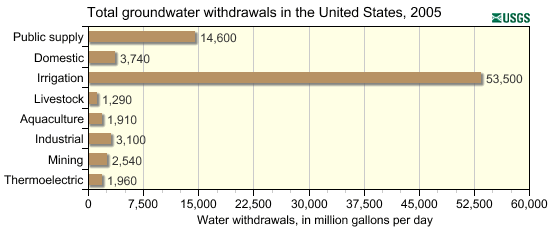
\includegraphics[scale=0.8]{figs/gwuse.png}
    \end{center}
\end{figure}
Most
notably, about 51\% of the total U.S. population and 99\% of the
rural population rely on groundwater as their drinking water
source~\cite{gw}. Unfortunately, by nature of being underground,
groundwater is highly susceptible to contaminants, e.g. fertilizers,
pesticides, road salt, gasoline, etc. Toxins that have leached into
the water supply have deleterious effects on human health as well as
serious environmental ramifications. 

We explore the characteristics of spatially perturbed one-dimensional
maps with the aim of understanding \textbf{in situ remediation} of contaminated
groundwater. In situ remediation involves injecting a treatment
solution in the groundwater to render the contaminants
inert. Degredation reactions require the two solutions be in close proximity to each other; the solutions must mix. Engineered Injection and Extraction (EIE)\footnote{EIE sequences are typically developed
heuristically to stretch and fold the fluid interface.} is an
approach that uses sequential injection and extraction of water in wells surrounding
the contaminated region to generate chaotic \textbf{advection}. A
solute is advected through a system when it moves with the local fluid
velocity~\cite{advection}. Degredation reactions are more efficient when the solutions are thoroughly mixed
together, so the onset of chaos in this system is a positive sign
because it indicates the interface length between the two reactants is
maximal, or at least large. The primary agent of mixing is the extent to which
solutions move underground (transmissivity)~\cite{neupauer}. 

Transmissivity, as a measure of how
much water may flow horizontally, is the governing property of the
degredation reactions because it limits the extent of chaotic advection. In turn, transmissivity depends on the type of sediment in
the aquifer because the sediment porosity is directly proportional to
hydraulic conductivity. For instance, clay typically has
very low hydraulic conductivity, but very high porosity (Table~\ref{tbl:porosity}). This
implies a section of the aquifer primarily made of clay can hold a
large volume of liquid per volume of sediment, but liquid flows slowly
through the region. Without the aid of sophisticated equipment to
determine the nature of the sediment underground, we might consider
the sediment to be randomly distributed in space. Therefore, the
spatial distribution of rocks and sediment plays an important role in the dynamics of the system. 

Exploring the dynamics of a one-dimensional system lays the groundwork
for understanding the dynamics of systems with higher dimensions. Two
one-dimensional systems known to exhibit chaotic behavior are the
logistic map and the circle map. Applying spatial perturbations to
these maps and observing the subsequent dynamics may give an
indication of what occurs in two-dimensional systems, like the
groundwater model. 

\section{Chaos}
One-dimensional maps, such as the logistic map and the circle map, are
analyzed in a variety of ways, e.g. fixed point iterations,
cobweb diagrams, bifurcation diagrams, etc. This section offers some
basic definitions and explanations of these concepts. One-dimensional maps are a
subclass of dynamical systems in which time is discrete, rather than
continuous. They take the form
\begin{equation*}
x_{n+1}=f(x_n),
\end{equation*}
where $x_n \in \mathbb{R}$ or $x_n \in \mathbb{S}^1$, the circle. These maps demonstrate that even simple dynamical systems are capable
of complex behavior, and as such, are also simple examples of chaos. 

The sequence of iterates ${x_0,x_1,...,x_n}$ in a map is
called an \textbf{orbit}. As $n \to \infty$, orbits may converge to a fixed point, a
set of periodic fixed points, or they may not converge at all. 

A \textbf{fixed point} $x^*$ of a function $f$ is an element of the
function's domain that is mapped to itself by the function, i.e.
\begin{equation*}
x^* = f(x^*).
\end{equation*}
In simple terms, a \textbf{periodic orbit} is an orbit that converges to a set
of points after many iterates. Consider the repeating sequence $\{z_m\}$
in an arbitrary closed orbit $\{x_n\}$, where $m,n \in \mathbb{N},
m<n$. The sequence $\{z_m\}$ may contain many terms, but since
$\{x_n\}$ is closed, $\{z_m\}$ eventually repeats. Thus, $z_{m+p}=z_m$
for some $p \in \mathbb{N}, p\geq 1$. If this is true for any $m \in
\mathbb{N}$, we call $p$ the period of the sequence, and $z_m$ the
period-$p$ point. If this is true only for $m > m_0$, then the
sequence $\{z_m\}$ is an
eventually periodic orbit.

Fixed points and periodic
orbits can be examples of attractors or repellors. An \textbf{attractor} has the following
properties: it is an invariant set, it attracts an open set of initial
conditions, and it is minimal~\cite{strogatz}. Since the attractor is
invariant, trajectories that begin in the attractor $A$ cannot escape
from $A$. By being minimal, we mean there does not exist a proper
subset of $A$ such that the previous two conditions are
satisfied. An attractor is considered chaotic if it is sensitive to
initial conditions. Otherwise, stable fixed points and periodic orbits are examples of attractors. Both types of attractors may have
a \textbf{basin of attraction}, which is the set $S=\{x_0:x(t) \to A, t \to \infty\}$, i.e.
the largest set of initial conditions $x_0$ that are drawn to the attractor as
time goes to infinity~\cite{strogatz}. The opposite of an attractor is
called repellor, a set that repels trajectories away from it.

Previously, we mentioned an attractor is considered chaotic if it
exhibits sensitive dependence on initial conditions, but in fact, the
definition of chaos is more complicated. Although no universal definition of chaos has been
agreed upon, the following working definition is generally acceptable~\cite{strogatz}:
\begin{singlespace}
\begin{definition}
Chaos is aperiodic long-term behavior in a deterministic
  system that exhibits sensitive dependence on initial conditions.
\end{definition}
\end{singlespace}
\begin{enumerate}
\item \textbf{Aperiodic long-term behavior} is another way of stating
  that there are trajectories within the map that do not limit to
  fixed points or more generally quasiperiodic orbits as $n \to \infty$.
\item \textbf{Deterministic} is used to describe systems in which a
  given state has exactly one orbit, i.e. there is no random input or parameter. The observed behavior of the
  system arises from its nonlinearity, not from random noise.
\item \textbf{Sensitive dependence on initial conditions} means that
  trajectories that start in almost the same place ($\epsilon$ apart)
  separate quickly. In most cases, this means the system has a
  positive Lyapunov exponent.
\end{enumerate}

\textbf{Lyapunov exponents} are a way of quantifying the sensitive
dependence on initial conditions for a specific orbit. If this limit
exists, Lyapunov exponents are defined as 
\begin{equation}\label{eq:lyap}
\lambda(x_0) = \lim_{n \to \infty} \frac{1}{n} \sum_{i=0}^{n-1} \ln |f'(x_i)|.
\end{equation}
For stable fixed points and stable periodic orbits, $\lambda(x_0) < 0$,
and for chaotic attractors, $\lambda(x_0)>0$. Equation~\ref{eq:lyap} essentially states that if the magnitude of the
derivative on the orbit is on average less than one (the logarithm
becomes negative), then there is no chaos. However, if the expansion
along the orbit is on average greater than one (the logarithm becomes positive), then it is a
sign of chaos. $\lambda(x_0)$ is the same for all initial conditions
$x_0$ in the same basin of attraction. 

The existence and stability of fixed points in $f$ are topics of great
interest as they constitute a major part in understanding the
dynamics of the map. If the domain is a complete metric space and $f$ is a contraction
mapping, the Contraction Mapping Theorem implies the map $f$ has a unique
fixed point~\cite{meiss}. We call a metric space $X$ \textbf{complete} if every
Cauchy sequence in $X$ converges to an element of $X$. A sequence is
Cauchy if the distance between any two elements of the sequence
approaches zero as we consider more and more terms of the
sequence. More formally, given a metric space $X$ with metric $\rho$, a sequence $f_n \in X$ is \textbf{Cauchy} if
$\forall \epsilon>0, \exists N(\epsilon)$ such that whenever $m,n \geq
N(\epsilon), \rho(f_n,f_m)<\epsilon$~\cite{meiss}. A metric measures
the distance between two elements of the space $f,g$, and must satisfy the following three
properties~\cite{meiss}:
\begin{enumerate}
\item Positivity. $\rho(f,g) \geq 0$ and $\rho(f,g)=0$ only when $f
  \equiv g$
\item Symmetry. $\rho(f,g) = \rho(g,f)$
\item Triangle inequality. $\rho(f,h) \leq \rho(f,g) + \rho(g,h)$
\end{enumerate}
A vector norm, such as the infinity norm, is an example of a metric. 
\begin{singlespace}
\begin{theorem}\label{thm:contraction}
The Contraction Mapping Theorem. Let $T:X\to X$ be a complete metric space $X$. If $T$ is a
contraction, i.e., if $\forall f,g \in X, \exists$ a constant $c<1$
such that $\rho(T(f),T(g)) \leq c\rho(f,g)$, then $T$ has a unique
fixed point, $f^* = T(f^*) \in X$.
%let $D$ be a closed, bounded and convex set in the plane. Assume the
% components of the iterative map $g(x)$ are continuously differentiable at all points of
% $D$, and further assume: 
% \begin{enumerate}
% \item $g(D) \subset D$
% \item $\lambda =\max_{x\in D}||G(x)||_\infty < 1$, where $G(x)$ is the Jacobian of
% $g(x)$
% \end{enumerate}
% Then, 
% \begin{itemize}
% \item $x=g(x)$ has a unique solution $\alpha \in D$
% \item For any initial point $x_0 \in D$, the iteration will converge
%   in $D$, i.e. $\lim_{t \to \infty}x_t = \alpha$
% \item $||\alpha - x_{n+1}||_\infty \leq
%   (\lambda +\epsilon_n)||\alpha - x_n||_\infty$ with
%   $\epsilon \to 0$ as $n\to \infty$
% \end{itemize}
\end{theorem}
\end{singlespace}

The stability of the fixed point $x^*$ is
determined by perturbing the fixed point by $\eta$ to see whether it is
attracted to or repelled from $x^*$. A Taylor series expansion around
the perturbation $x_{n+1} = x^* + \eta_{n+1}$ linearizes the map
\begin{align*}
\begin{split}
x^* + \eta_{n+1} &= f(x^* + \eta_n)\\
&= f(x^*) + f'(x^*)\eta_n + \mathcal{O}(\eta_n^2),\\
\eta_{n+1} &= f'(x^*)\eta_n + \mathcal{O}(\eta_n^2).\\
\end{split}
\end{align*}
Neglecting the higher order terms in $\mathcal{O}(\eta_n^2)$ leaves
$\eta_{n+1} = f'(x^*)\eta_n$. The multiplier is $\hat{\lambda} =
f'(x^*)$. Solutions of the map are found by extending the recursion
\begin{align*}
\begin{split}
\eta_{1} &= \hat{\lambda}\eta_0\\
\eta_{2} &= \hat{\lambda}\eta_1 = \hat{\lambda}^2\eta_0\\
&...\\
\eta_{n} &=\hat{\lambda}^n\eta_0.
\end{split}
\end{align*}
If $|\hat{\lambda}| = |f'(x^*)| > 1$, $\lim_{n \to \infty}\hat{\lambda}^n = \infty$, and
the fixed point $x^*$ is \textbf{linearly unstable}. If $|\hat{\lambda}| = |f'(x^*)| < 1$, $\lim_{n \to
  \infty}\hat{\lambda}^n = 0$, and the fixed point $x^*$ is
\textbf{linearly stable}. If
$|\hat{\lambda}| = |f'(x^*)| = 1$ the $\mathcal{O}(\eta_n^2)$ terms
determine the local stability~\cite{strogatz}. 

Likewise, a Taylor expansion about a periodic orbit demonstrates its
stability criteria. Suppose we have a period 2 orbit. This implies
$f(u)=v$ and $f(v)=u$. Both $v,u$ are solutions of $f \circ
f= f^2(x) = x$, so $v,u$ are fixed points of $f^2(x)$. We compute the
multiplier $\hat{\lambda}$,
\begin{align*}
\begin{split}
\hat{\lambda} &= \frac{d}{dx} f(f(x)) \\
&= f'(f(x))f'(x).
\end{split}
\end{align*}
Evaluating the multiplier at $x=v$ yields
\begin{align*}
\hat{\lambda} = f'(u)f'(v).
\end{align*}
By the symmetry of the final product, evaluating the multiplier at
$x=u$ returns the same multiplier. Furthermore, we can generalize the
stability analysis of a periodic orbit of order $p$. Each point of a
periodic orbit $u_1,u_2,...u_p$ is a fixed point of the map
$f^p(x)$. Interestingly, any one of the points $u_j$ may be a fixed point or a point
on another periodic orbit of period less than $p$, e.g., a fixed
point $x^*$ of $f$ is also the root of $f^p(x)-x$ for any $p$. We
calculate the multiplier and evaluate along the points of the orbit,
$u_j$, finding
\begin{align*}
\begin{split}
\hat{\lambda} &= \frac{d}{dx} f^p(x) \\
&= \left(\frac{d}{dx} f^p(x)\right) \left(\frac{d}{dx} f^{p-1}(x)\right) ... \left(\frac{d}{dx} f(x)\right)\\
&...\\
&= f'(u_p)f'(u_{p-1})...f'(u_{2})f'(u_{1}).
\end{split}
\end{align*}
The magnitude of the multiplier can take on values
\begin{displaymath}
|\hat{\lambda}| =  \prod_{j = 1}^{p}|f'(u_j)| =\left\{
     \begin{array}{lr}
       <1 & \\
       =1 & \\
       >1 & .\\
     \end{array}
   \right.
\end{displaymath} 
As in the fixed point scenario, $|\hat{\lambda}|<1$ implies the orbit
is stable, the $\mathcal{O}(\eta_n^2)$ terms of the Taylor
expansion determine the local stability for $|\hat{\lambda}|=1$, and $|\hat{\lambda}|>1$ corresponds to an unstable
orbit. However, the difference lies in the fact that the
stability of the orbit depends on the derivative at all points on the
orbit. In other words, if there is a point along the orbit where the
slope is extremely large, then it is possible the orbit is unstable. 

Linear stability is
linked to nonlinear stability by the Hartman-Grobman
Theorem~\cite{meiss}. The Hartman-Grobman theorem states the behavior of the linearized
dynamical system near a fixed point is topologically equivalent to the
behavior of the nonlinear system near the same point, as long as the
multiplier $|\hat{\lambda}|\neq 1$. The term \textbf{topologically
  equivalent} means that there is a homeomorphism, or a continuous and
invertible map, between the linear and nonlinear system such that the
directions of the trajectories are preserved~\cite{strogatz}. Therefore, the results of linear stability
analysis of fixed points and orbits translates to nonlinear stability. 

Fixed points may be created, destroyed, or their stability may
change. Such a qualitative change in dynamics is called a \textbf{bifurcation}~\cite{strogatz}. These changes are strongly dependent on the
parameters of the system. There are many types of
bifurcations, such as~\cite{strogatz}: 
\begin{enumerate}
\item saddle-node\footnote{Also called a fold bifurcation, a
    turning-point bifurcation, or a blue-sky bifurcation.}: As a parameter increases or decreases, two fixed
  points approach one another, collide, and finally are destroyed. The
  reverse may also occur, where the system begins with no fixed
  points, then one is created, and finally it splits into two points. 
\item transcritical: No matter how a parameter varies, there is no
  creation nor destruction of fixed points. However, the stability of
  the fixed point may change between stable, semistable, and unstable. In all cases, it
  exchanges stability with another fixed point. 
\item pitchfork: Fixed points appear and disappear in
  symmetrical pairs as a parameter is varied. There are two types of
  pitchfork bifurcations:
\begin{enumerate} 
\item supercritical pitchfork\footnote{Sometimes referred to as a
    forward, soft or safe bifurcation.}: One stable fixed point splits into
  three points after the bifurcation: a pair
  of stable fixed points that flank one unstable fixed point, located
  where the original stable fixed point was. 
\item subcritical pitchfork\footnote{Can be called an inverted,
    backward, hard, or dangerous bifurcation.}: A pair of unstable fixed points exists only below
  the bifurcation. The pair also flanks one stable fixed point, which
  becomes unstable after the bifurcation.
\end{enumerate}
\item period-doubling\footnote{Also known as a flip bifurcation.}:
  When a parameter increases past a certain point, a stable periodic orbit of
  order $2p$ appears near an orbit of order $p$, and the orbit of
  order $p$ looses stability. One mechanism for the creation of chaos is if
  an infinite sequence of period-doubling bifurcations occurs. 
\end{enumerate}
A bifurcation diagram is a
visual demonstration of the change in dynamics of a system as its
parameters are varied. Bifurcation diagrams are constructed by
plotting the qualitative behavior of the orbits of a map as a function of its
parameters, such as the locations of the stable and unstable orbits as
a function of the parameters of the map. 

A \textbf{cobweb diagram} is a graphical representation of the orbit
iterations. The method of the cobweb diagram can be outlined in four
steps, and is depicted in Figure~\ref{fig:cobex}.
\begin{figure}[!h]
\caption[Example of a Cobweb Diagram]{A one-dimensional map (blue) and
  the line $x_{n+1}=x_n$ (red) with a few iterates of the cobweb
  diagram (green). Cobweb diagrams encapsulate the dynamics of the orbit at a glance.}\label{fig:cobex}
    \begin{center}
	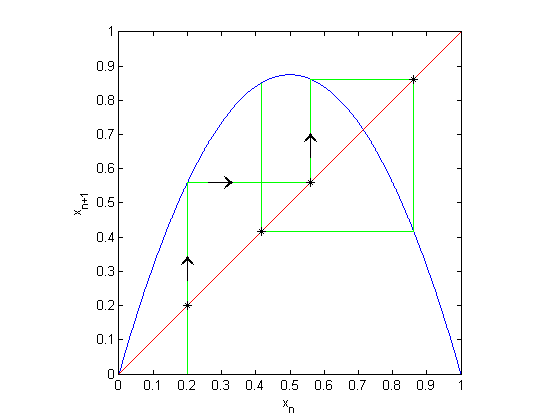
\includegraphics[scale=0.8]{figs/cobweb_ex.png}
    \end{center}
\end{figure}

\begin{enumerate}
\item Begin at the Cartesian coordinate pair $(x_0, f(x_0))$, which
  may also be written as $(x_0, x_1)$
\item Plot horizontally the distance from $(x_0, f(x_0)=(x_0, x_1)$ to $(f(x_0),
  f(x_0))=(x_1, x_1)$
\item Plot vertically from $(f(x_0), f(x_0))=(x_1, x_1)$ to $(f(x_0), f(f(x_0)))=(x_1, x_2)$
\item Repeat steps 2-3 until convergence or divergence is determined
  (or perhaps the maximum number of iterations has been reached):
  $(x_n, x_{n+1}) \to (x_{n+1}, x_{n+1}) \to (x_{n+1},x_{n+2})$
\end{enumerate}

\subsection{Logistic Map}
The Logistic map is a quadratic recursive equation that maps the domain
$[0,1] \rightarrow [0,1]$. It is a commonly studied example in nonlinear dynamics and has
applications in population modeling. Robert May popularized the
logistic map in 1976~\cite{may}. He demonstrated that even simple nonlinear
maps could have complicated dynamics. There is one parameter in the
expression, $r$, which can take any value in the range [0,4] so that
[0,1] is an invariant set of the map. We define the map $f:[0,1]\to [0,1]$
\begin{equation}\label{logmap}
x_{n+1} = f(x_n) = rx_n(1-x_n).
\end{equation}
For a fixed initial condition $x_0$ and $r$, the long term behavior of
the map may be obtained by iteration, using~(\ref{logmap}). 
\begin{figure}[!h]
\caption[Deterministic logistic map, stable orbit]{Deterministic
  Logistic Map (blue) for $r=3.2$. There is a stable period 4
  orbit. The period is calculated by counting the number of crossings
  from the cobweb diagram (green) on the line $x_{n+1}=x_n$ (red). The
  transient iterations were removed to make demonstrate the long-term
  behavior of the orbit.}\label{fig:detlogstable}
    \begin{center}
	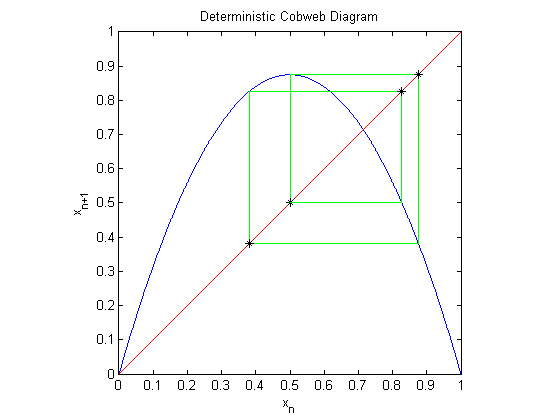
\includegraphics[scale=0.75]{figs/det_cobweb.png}
    \end{center}
\end{figure}
For example, Figure~\ref{fig:detlogstable}
demonstrates a stable period 4 orbit, whereas Figure~\ref{fig:detlogunstable}
demonstrates a possibly chaotic orbit. 
\begin{figure}[!h]
\caption[Deterministic logistic map, unstable orbit]{Deterministic
  Logistic Map (blue) for $r=3.8$. There appears to be no
  stable orbit. The cobweb diagram (green) behaves erratically, even
  after removing the transient behavior. For values of $r \in
  [3.5,4]$, the system is chaotic.}\label{fig:detlogunstable}
	\begin{center}
		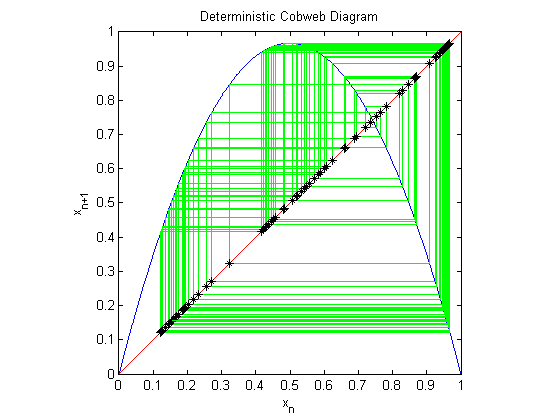
\includegraphics[scale=0.75]{figs/chaos.png}
	\end{center}
\end{figure} 
The effects of the parameter $r$ are
tabulated in Table~\ref{tbl:bif} and also graphically visualized in
Figure~\ref{fig:bif}, a bifurcation diagram. 
\begin {table}[!h]
\begin{center}
\caption[Behavior of the deterministic map as $r$ is varied]{As $r$ is
varied over [0,4], the logistic map undergoes notable changes in terms
of stability~\cite{may}.}\label{tbl:bif}
\begin{tabular}{ | p{4cm}| p{8cm}|}   \hline
$r \in [0,1]$ & convergence to the stable Period
1 orbit, $x=0$ \\ \hline
$r \in [1,2]$ & convergence to the stable Period 1
orbit, $x = \frac{r-1}{r}$\\ \hline
$r \in [2,3]$ & convergence to the stable Period 1
orbit, $x = \frac{r-1}{r}$, but at a slower rate\\ \hline
$r \in [3,3.44949]$ & emergence of stable Period 2 orbits\\ \hline
$r \in (3.44949, 3.54409)$ & emergence of stable Period 4 orbits\\ \hline
$r \in [3.54409,3.56995)$ & period doubling cascade\\ \hline
$ r \approx 3.56995 $ & onset of chaos\\\hline
$r \in (3.56995,4]$ & mostly chaotic behavior, but there are islands of
stability (eg. Period 3 orbits for $r \approx 3.82843$) \\\hline
\end{tabular}
\end{center}
\end {table}
Most notably, there is no chaos for values of $r
< 3.5$, and for $r > 3.5$, the system often appears chaotic, although
there are islands of stability interspersed throughout the bifurcation
diagram. The Lyapunov exponent $\lambda$ of the logistic map is an indicator of
chaos. Figure~\ref{fig:detloglyap} demonstrates how the Lyapunov
exponent of the logistic map changes sign as a function of
$r$. $\lambda$ approaches zero at the period-doubling bifurcations
shown in Figure~\ref{fig:bif}. The negative spikes in the plot around
$r=3.2$ and $r=3.5$ correspond to the period 2 and period 4 orbits in the
bifurcation diagram. In fact, $\lambda = -\infty$ when $f'(x_j)=0$ for some $x_j$,
and such orbits are called \textbf{superstable orbits}. Chaotic behavior appears where $\lambda >0$, near
$r=3.57$. The islands of stability in the bifurcation diagram are
visible where $\lambda$ dips past zero, notably around $r=3.83$.
\begin{figure}[!h]
\caption[Bifurcation diagram for the deterministic logistic map]{The
  behavior in Table~\ref{tbl:bif} may be graphed in a bifurcation
  diagram, there the long term behavior of the map is a function of $r$. The left diagram ranges from $r\in
  [0,4]$, and the right diagram ranges from $r\in [2.5,4]$. Notice the
  islands of stability in the chaotic region of the map.}\label{fig:bif}
\centering
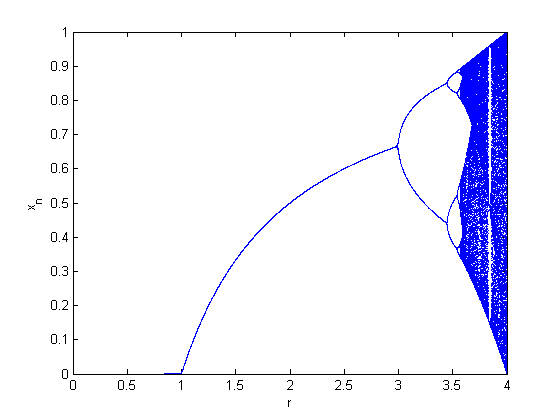
\includegraphics[width=.5\textwidth]{figs/det_bif_1.png}\hfill
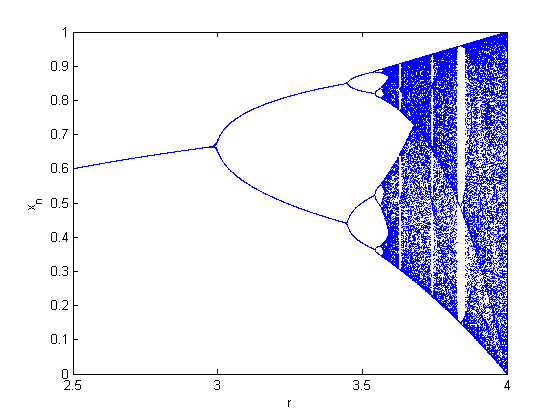
\includegraphics[width=.5\textwidth]{figs/det_bif_2.png}
\end{figure}
\begin{figure}[!h]
\caption[Lyapunov exponent in the deterministic logistic map]{The
  Lyapunov exponent for the deterministic
  logistic map, where $x_0=0.7$ for $r \in
  [3,4]$. The positive values of $\lambda$ for $r>3.57$ indicate the system is chaotic.}\label{fig:detloglyap}
	\begin{center}
		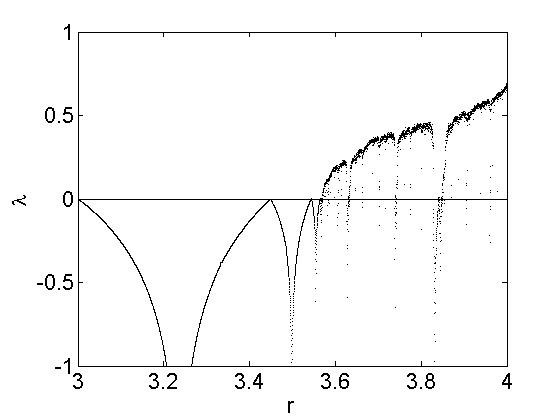
\includegraphics[scale=0.65]{figs/det_log_lyap.png}
	\end{center}
\end{figure} 

\subsection{Circle Map}
The circle map is another
dynamical system whose deceivingly simple form gives way to complicated behavior. It was used to
understand the dynamics of a kicked rotor by Vladimir
Arnold, who is credited for discovery of what are now called the Arnold Tongues, which are
regions of stable periodic motion in the bifurcation diagram of the
map. Generally, a degree-one circle map takes the form
\begin{align*}
x_{n+1}&=f(x)=x_n + \omega + g(x_n) \mod 1\\
g(x_n)&=g(x_n + 1),
\end{align*}
where the angle $x$ has been normalized so that its range is $[0,1)$
instead of $[0,2\pi )$, $\omega$ is the natural frequency of the map, and
$g(x)$ is the nonlinear component of the recursion~\cite{rasband}. The
parameter $\omega$ represents the natural frequency of the rotor, and
$g$ models the driving force with period 1 in time. We define the circle $S^1$ as $\mathbb{R} \setminus
\mathbb{Z}$. The \textbf{degree} of a map $f:S^1 \to S^1$ is the integer
deg($f$) given by 
\begin{align*}
\deg(f) = F(1) - F(0),
\end{align*}
where $F:\mathbb{R} \to \mathbb{R}$ is the lift of the
map. $F$ is called the \textbf{lift} of $f$ if
\begin{align*}
w \circ F = f \circ w,
\end{align*}
where $w:\mathbb{R} \to S^1$ is defined as
\begin{equation*}
w(x) = e^{2\pi i x} = \cos(2\pi x) + i\sin(2\pi x).
\end{equation*}
$w$ wraps $\mathbb{R}$ around the circle $S^1$ without critical
points~\cite{devaney}. $w$ is many-to-one, therefore it is not a
topological conjugacy (homeomorphism)
between $F$ and $f$. When $f$ is an orientation
preserving diffeomorphism of the circle, the lift of $f$ must be
monotonic increasing, i.e. $F'(x)>0$. A function is a \textbf{diffeomorphism}
if it is a smooth, differentiable, invertible map between two or more
manifolds. The term \textbf{topologically conjugate} means that there
is a homeomorphism (a continuous and invertible function whose inverse
is also continuous)
that transforms one map to another in such a way that the sense of
time is preserved~\cite{strogatz}.

\begin{singlespacing}
\begin{definition}
Let $f:I \to J$. The function $f(x)$ is a homeomorphism if $f(x)$ is
one-to-one, onto, and continuous, and $f^{-1}(x)$ is also continuous~\cite{devaney}.
\end{definition}
\begin{definition}
Let $f:I\to J$. The function $f(x)$ is a $C^r$-diffeomorphism if
$f(x)$ is a $C^r$-homeomophism such that $f^{-1}(x)$ is also $C^r$~\cite{devaney}. 
\end{definition}
\end{singlespacing}

Arnold introduced the two-parameter example
\begin{align}\label{detcirc}
x_{n+1}= F(x_n) =  x_n + \omega - \frac{k}{2\pi}\sin(2\pi x_n),
\end{align}
which we will explore as well. Equation (\ref{detcirc}) is the lift of the map
$f$,
\begin{align}\label{detcirc2}
f(x_n) = x_n + 2\pi \omega - \frac{k}{2\pi}\sin(2\pi x_n) \mod 1.
\end{align}
Taking the modulus of~(\ref{detcirc}) maps the circle
to itself. In both (\ref{detcirc}) and (\ref{detcirc2}), there are two parameters: $k \in [0,\infty)$
is the coupling strength and $\omega \in [0,1]$ is the driving
frequency. A stable period 2 orbit is shown in
Figure~\ref{fig:dcircstable}, and
Figure~\ref{fig:rcircunstable} shows an orbit that appears to be quasiperiodic.
\begin{figure}[!h]
\caption[Deterministic circle map, stable orbit]{The cobweb
  diagram (green) for a deterministic circle map (blue) with $\omega =
  0.5$ and $k=1$. After 1000 iterations, we see a stable period 2 orbit. Transient iterations were removed.}\label{fig:dcircstable}
	\begin{center}
		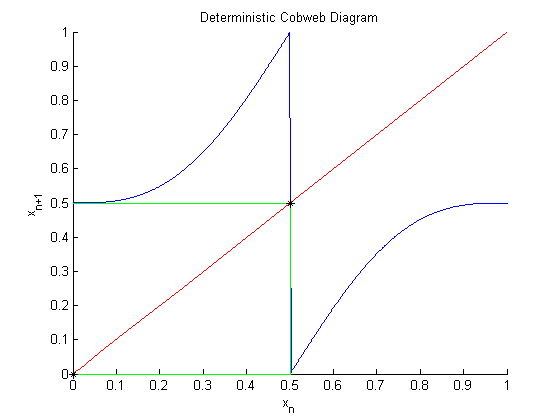
\includegraphics[scale=0.7]{figs/detcirc_cobweb_2.png}
	\end{center}
\end{figure}
\begin{figure}[!h]
\caption[Deterministic circle map, quasiperiodic orbit]{The cobweb
  diagram (green) for a deterministic circle map (blue) with $\omega =
  0.6$ and $k=1$. After 1000 iterations, we see a possibly quasiperiodic orbit. Transient iterations were removed.}\label{fig:rcircunstable}
	\begin{center}
		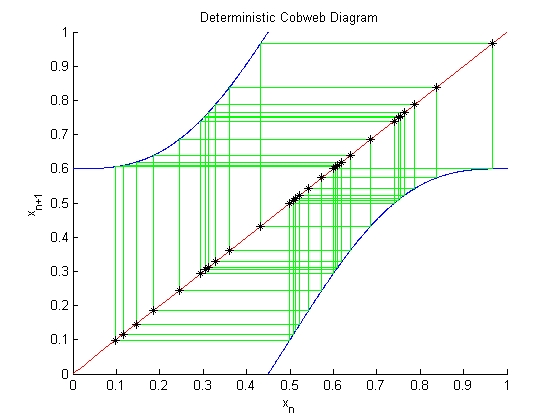
\includegraphics[scale=0.7]{figs/detcirc_cobweb_chaos.png}
	\end{center}
\end{figure}
When discussing $f$, we will deal exclusively with the
lift, $F$.

The coupling strength $k$ controls the amplitude of the oscillations in the circle map; no
coupling is $k=0$, and the coupling increases as $k \to
\infty$. For $-1 \leq k < 1$, $f$ is a diffeomorphism of $S^1$, and
when $|k|=1$, the map is a homeomorphism. $f$ is monotone only if
$|k|\leq 1$. For $k>1$, the map is no
longer one-to-one. In contrast, $\omega$
applies a positive vertical shift to the map, which causes the map to wrap
around itself, due to the effects of the modulo operator. 

A phenomenon of \textbf{mode-locking} may occur in the lift of the map,
where after $q$ iterations, the new angle differs from the initial
value of $x$ by exactly $p \in \mathbb{Z}$
\begin{align*}
x_{n+q}=x_n+p.
\end{align*}
The mode-locked state of the lift $F$ implies the orbit is periodic
on $\mathbb{S}^1$, i.e. $x_{n+p} \mod 1 = x_n \mod 1$. The \textbf{rotation number} of the orbit is an important invariant of
the circle map because it measures the average amount a point is rotated per iteration of the map. Essentially, it gives an idea of
whether $f$ has periodic orbits in $\mathbb{S}^1$.

\begin{singlespacing}
\begin{definition}\label{rho}
The rotation number of $f$, $\rho(f)$, is the fractional part of
$\rho_0(F) = \lim_{n \to \infty} \frac{|F^n(x)|}{n}$ for any lift $F$ of $f$. That is, $\rho(f)$ is the unique
number in [0,1) such that $\rho_0(F)-\rho(f)$ is an integer~\cite{devaney}.
\end{definition}
\end{singlespacing}

\noindent It is important that $\rho(f)$ depends only on $f$ when $f$
is a homeomorphism. But, if not, it can depend on $x$ as well. Recall when $|k|>1$,
the map~(\ref{detcirc}) is no longer one-to-one, so $\rho$
may not exist~\cite{devaney}. When $\rho \in \mathbb{Q}$, the system is mode-locked. Since
$\rho$ is a rational number, it can be expressed as $p/q$, where $p,q
\in \mathbb{Z}$. The order of the periodic orbit is $q$. If $\rho$
does not exist (when $f$ is not a homeomorphism), then the system may be in a chaotic
state. When $f$ is a homeomorphism and $\rho \in \mathbb{R} \setminus
\mathbb{Q}$, the orbit is quasiperiodic. Quasiperiodicity refers to irregular periodicity in the
system; the periodicity does
not occur at regular intervals. The changes in the rotation number $\rho$ as $\omega$ is
varied over [0,1] is graphically demonstrated as a devil's staircase
in Figure~\ref{fig:devil_det}. 
\begin{figure}[!h]
\caption[The devil's staircase for the deterministic circle map]{The devil's
  staircase. For $|k| \leq 1$, $f$ is a homeomorphism, so the
  staircase is monotone. The largest steps (where $\rho$ appears
  constant) correspond with the simplest rationals. If $|k|>1$, $f$ is
  not a homeomorphism so $\rho$ may not exist. In all plots, $\omega \in [0,1],\Delta \omega = 0.001$}\label{fig:devil_det}
	\begin{center}
		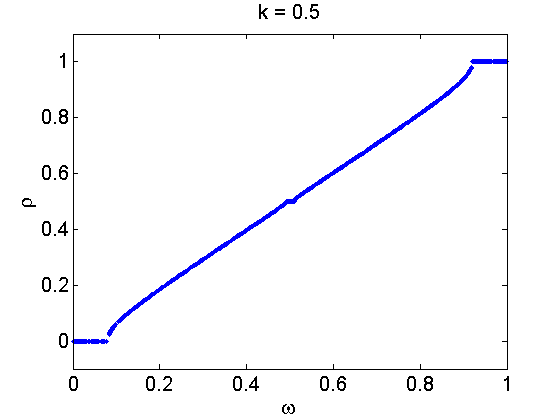
\includegraphics[width=.33\textwidth]{figs/detcirc_devil_k05.png}\hfill
		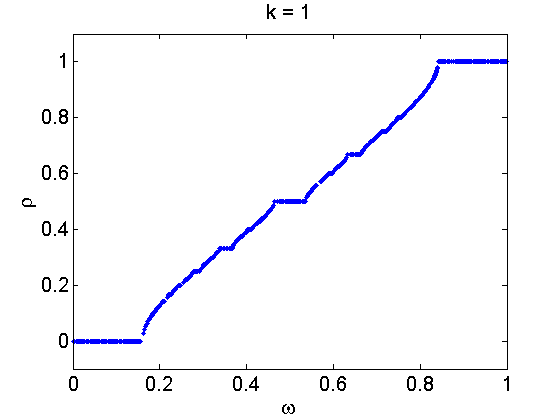
\includegraphics[width=.33\textwidth]{figs/detcirc_devil_k1.png}\hfill
		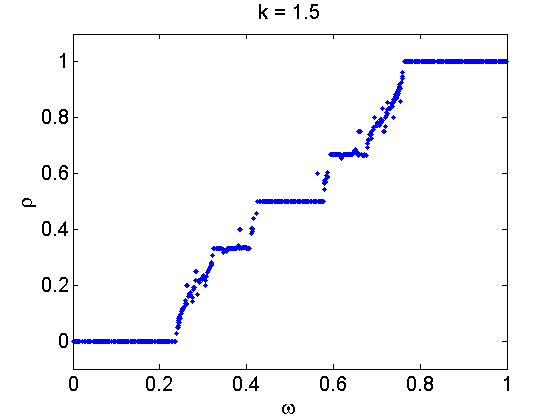
\includegraphics[width=.33\textwidth]{figs/detcirc_devil_k15.png}
	\end{center}
\end{figure}
The devil's staircase a monotone
function that is constant at rational rotation numbers, and takes on
every value in between the rational numbers~\cite{devaney}. Interestingly, the graph of $\rho(\omega)$ is a Cantor
function. Cantor functions are everywhere continuous and monotone, but have zero
derivative almost everywhere. 

The theorem below
establishes that the rotation number of the map $\rho(f)$
depends continuously on $f$, and that if $f$ is monotone, then all
orbits have the same rotation number.

\begin{singlespacing}
\begin{theorem}
Let $f:S^1 \to S^1$ be an orientation-preserving diffeomorphism with
lift $F$. Then
\begin{equation*}
\rho_0(F) = \lim_{n \to \infty} \frac{|F^n(x)|}{n}
\end{equation*}
exists and is independent of $x$ and $\rho$ is independent of the lift $F$. Hence the
rotation number $\rho(f)$ is well-defined~\cite{devaney}.
\end{theorem}
\end{singlespacing}

The width of each ``step" in the devil's staircase corresponds to the width of the Arnold
tongues (Figure~\ref{fig:dettongues}) in the bifurcation diagram for
$k$ and $\omega$ in~(\ref{detcirc}). The colored
triangular regions in Figure~\ref{fig:dettongues} resemble tongues,
and are aptly named as such.
\begin{figure}[!h]
\caption[The Arnold Tongues for the deterministic circle map]{A color coded
  plot of the Arnold Tongues in the circle map. This plot samples 1000 values of $\omega
  \in [0,1]$ and $k \in
  [0,1.5]$, and checks for periodicity up to period 100. The colorbar
  to the right demonstrates the period order and corresponding
  color.}\label{fig:dettongues}
	\begin{center}
		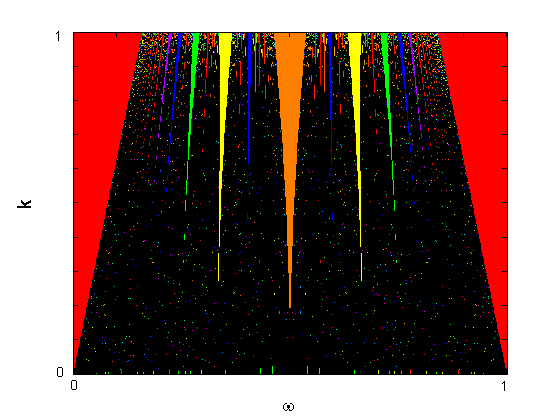
\includegraphics[scale=0.45]{figs/tongues_1000_det.png}
	\end{center}
\end{figure}
Recall the onset of chaos is marked by a positive Lyapunov
exponent. Figure~\ref{fig:detcirclyap} shows the Lyapunov exponent
$\lambda$ of
the circle map as a function of $\omega$ for $k=1.5$. Although small in
magnitude, $\lambda$ fluctuates between negative and positive
values around the Arnold tongues. The negative stretches in $\lambda$
coincide with the periodic fixed points in Figure~\ref{fig:dettongues}.  
\begin{figure}[!h]
\caption[Lyapunov exponent in the deterministic circle map, varying $\omega$]{The
  Lyapunov exponent for the deterministic
  circle map, where $k=1.5,x_0=0.7$. The positive values of $\lambda$
  indicate the system may be chaotic. About 10,000 values of $\lambda$
were computed over $\omega \in [0,1]$.}\label{fig:detcirclyap}
	\begin{center}
		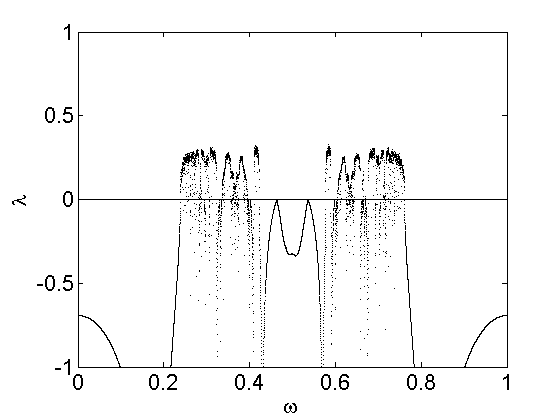
\includegraphics[scale=0.55]{figs/det_circ_lyap.png}
	\end{center}
\end{figure} 
Figure~\ref{fig:detcirclyapk} demonstrates chaotic behavior occurs
when $k > 1$.
\begin{figure}[!h]
\caption[Lyapunov exponent in the deterministic circle map, varying $k$]{The
  Lyapunov exponent for the deterministic
  circle map, where $\omega=0.7,x_0=0.7$. About 10,000 values of $\lambda$
were computed over $k \in [0,5]$.}\label{fig:detcirclyapk}
	\begin{center}
		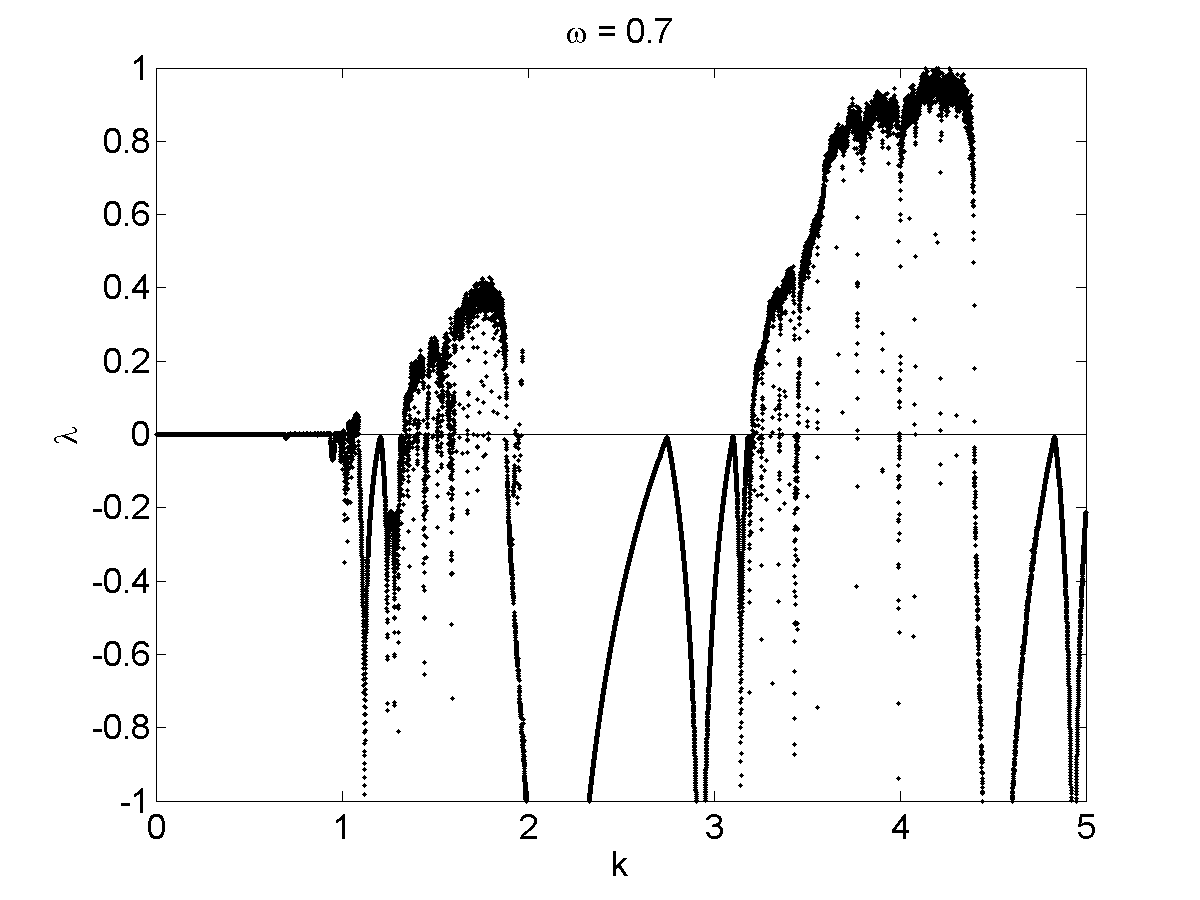
\includegraphics[scale=0.45]{figs/det_circ_lyap_k.png}
	\end{center}
\end{figure} 
